\documentclass[12pt]{article}

% TEMPLATE DEFAULT PACKAGES
\usepackage{amssymb,amsmath,amsfonts,eurosym,geometry,ulem,graphicx,color,setspace,sectsty,comment,natbib,pdflscape,array,adjustbox}

% ADDED PACKAGES FOR THIS MANUSCRIPT
\usepackage{palatino,newtxmath,multirow,titlesec,threeparttable,tabu,booktabs,titlesec,threeparttable,mathtools,bm,bbm,subcaption,pdflscape,tcolorbox,mathrsfs}
% endfloat,

\usepackage{afterpage}
\usepackage[hyphens]{url}
\usepackage[margin=1cm]{caption}

\usepackage[draft]{hyperref}
\newcommand{\tim}{$\,\times\,$}
% FIGURES & TABLES CAPTION STYLING
\captionsetup[figure]{labelfont={bf},name={Figure},labelsep=period}
\captionsetup[table]{labelfont={bf},name={Table},labelsep=period}

% SECTION TITLE SETTINGS
\titlelabel{\thetitle.\enskip}
\titleformat*{\section}{\large\bfseries}
\titleformat*{\subsection}{\normalsize\bfseries}

% COLUMN TYPES
\newcolumntype{L}[1]{>{\raggedright\let\newline\\\arraybackslash\hspace{0pt}}m{#1}}
\newcolumntype{C}{>{\centering\arraybackslash}p{5.2em}}
\newcolumntype{D}{>{\centering\arraybackslash}p{5em}}
\newcolumntype{R}[1]{>{\raggedleft\let\newline\\\arraybackslash\hspace{0pt}}m{#1}}


% MARGINS AND SPACING
\normalem
\geometry{left=1.1in,right=1.1in,top=1.0in,bottom=1.0in}
\setlength{\parskip}{2.5pt}

% SPECIAL CELL 
\newcommand{\specialcell}[2][c]{%
	\begin{tabular}[#1]{@{}l@{}}#2\end{tabular}}

% NO INDENT ON FOOTNOTES
\usepackage[hang,flushmargin]{footmisc}

\begin{document}



\vspace{0mm}
\begin{table}[h!]
\centering
\caption{Housing Project Areas Description}\label{table:projectdescriptives}
\vspace{0mm}
\begin{tabular}{l*{1}{cccccc}}
\toprule
  & \multicolumn{2}{c}{\textbf{All}}& \multicolumn{2}{c}{\textbf{Greenfield}}  & \multicolumn{2}{c}{\textbf{In-Situ}}   \\
  &Const. & Unconst. &Const. & Unconst.   & Const. & Unconst. \\
\midrule
 Number of Projects  & 172  & 145  & 43  & 20  & 27  & 29  \\ 
 Area (km2)  & 1.17  & 1.16  & 1.72  & 2.42  & 1.50  & 0.88  \\ 
 Median Construction Yr.  & 2006  & 2006  & 2006  & 2005  & 2004  & 2006  \\ 
 Delivered Houses  & 374  & 11  & 568  & 24  & 702  & 20  \\ 
 House Price in 1 km (R$^\dagger$)  & 188,441  & 218,635  & 194,214  & 186,841  & 179,596  & 208,570  \\ 
 Distance to CBD$^\ddagger$ (km)  & 32.5  & 27.7  & 40.5  & 39.9  & 32.6  & 30.6  \\ 

\bottomrule
\multicolumn{7}{l}{\scriptsize Const. refers to constructed projects and unconst. refers to unconstructed projects.}\\[-.5em]
\multicolumn{7}{l}{\scriptsize $^*$Calculated from {\it expected} completion dates using Gauteng National Treasury budget reports.}\\[-.5em]
\multicolumn{7}{l}{\scriptsize $^\dagger$ The USD averaged to about 7.70 Rands during the 2001-2011 period.}\\[-.5em]
\multicolumn{7}{l}{\scriptsize $^\ddagger$Measured as the average minimum distance with respect to Johannesburg and Pretoria CBDs. } \\[-.5em]
%\multicolumn{7}{l}{\scriptsize City includes projects whose centroids are within 30.4 km of their nearest CBD.} \\[-.5em]
%\multicolumn{7}{l}{\scriptsize Suburb includes projects whose centroids are further than 30.4 km from their nearest CBD.}
\end{tabular}
\end{table} 



\begin{figure*}
        \centering
   %     \caption[ Pre-Period Housing Densities in Constructed and Unconstructed Projects Areas ]
  %      {\small Pre-Period Densities} 
        %\vspace{2mm}
        \begin{subfigure}[b]{0.48\textwidth}
                    \caption[Network2]%
            {{\footnotesize \textbf{All Projects} pre-period formal raw data}}    
            \label{fig:prefor}
            \centering
            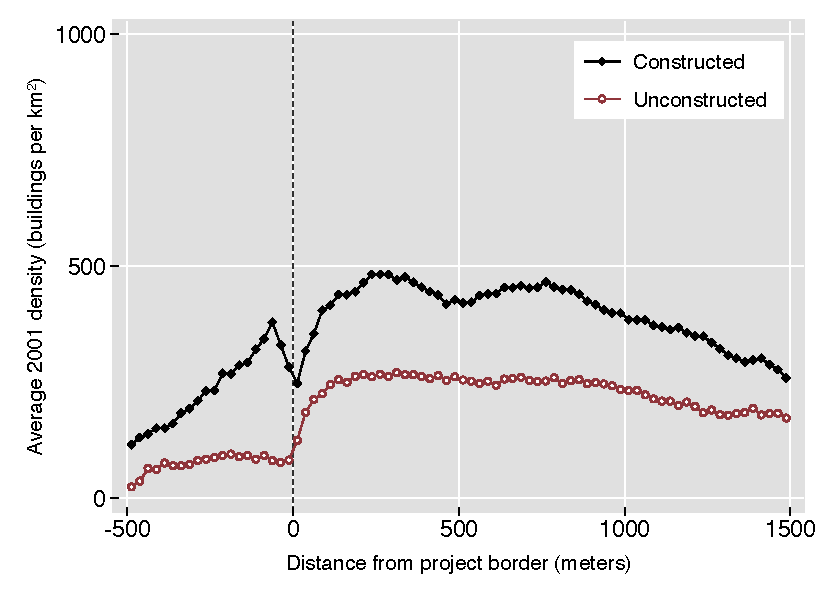
\includegraphics[width=\textwidth,trim={0.3cm .3cm 0.1cm 0cm}, clip=true]{figures/bblu_for_pre_means_4_spk.pdf}

        \end{subfigure}
        \hfill
        \begin{subfigure}[b]{0.48\textwidth}  
                    \caption[]%
            {{\footnotesize \textbf{All Projects} pre-period informal  raw data}}      
            \label{fig:preinf}
            \centering 
            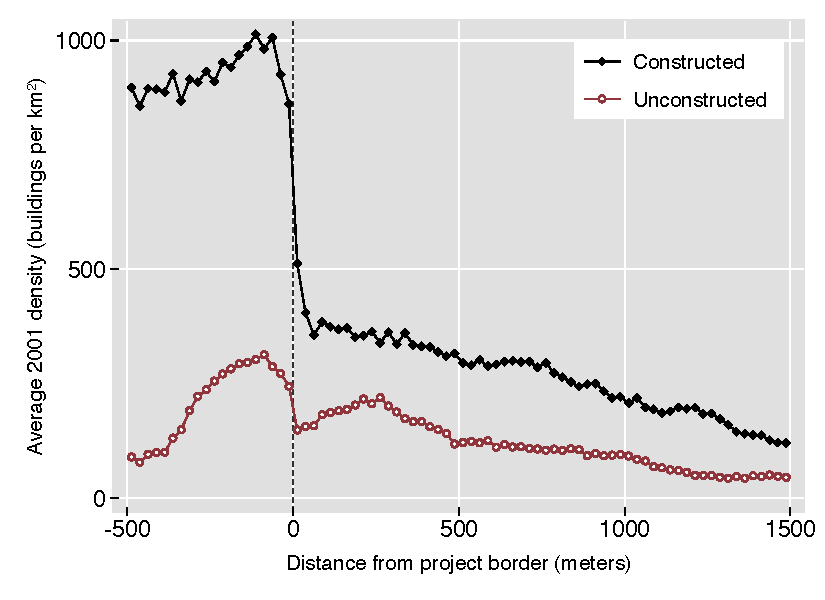
\includegraphics[width=\textwidth,trim={0.3cm .3cm 0.1cm 0cm}, clip=true]{figures/bblu_inf_pre_means_4_spk.pdf}

        \end{subfigure}
        \begin{subfigure}[b]{0.48\textwidth}
                    \caption[Network2]%
            {{\footnotesize \textbf{Greenfield} pre-period formal  raw data}}    
            \label{fig:prefor}
            \centering
            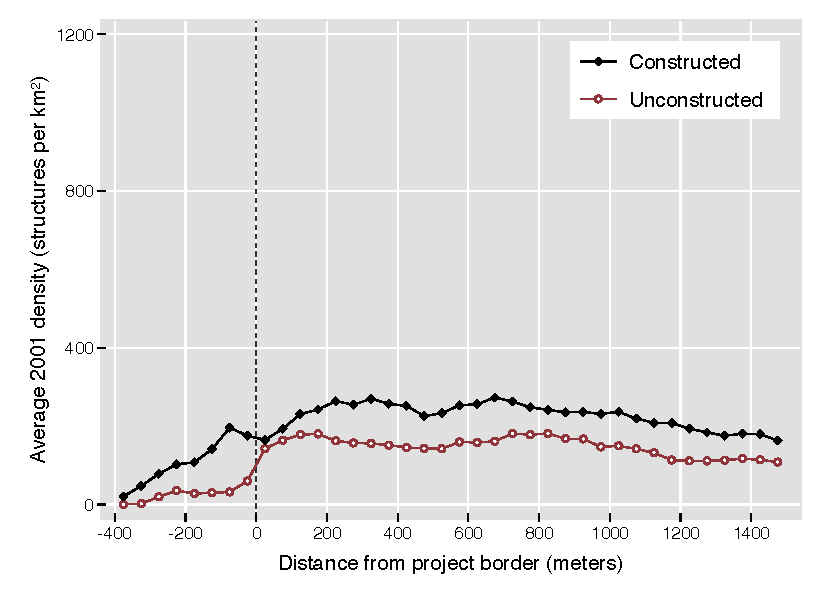
\includegraphics[width=\textwidth,trim={0.3cm .3cm 0.1cm 0cm}, clip=true]{figures/bblu_for_pre_means_4_1_spk.pdf}

        \end{subfigure}
        \hfill
        \begin{subfigure}[b]{0.48\textwidth}  
                    \caption[]%
            {{\footnotesize \textbf{Greenfield} pre-period informal  raw data}}     
            \label{fig:preinf}
            \centering 
            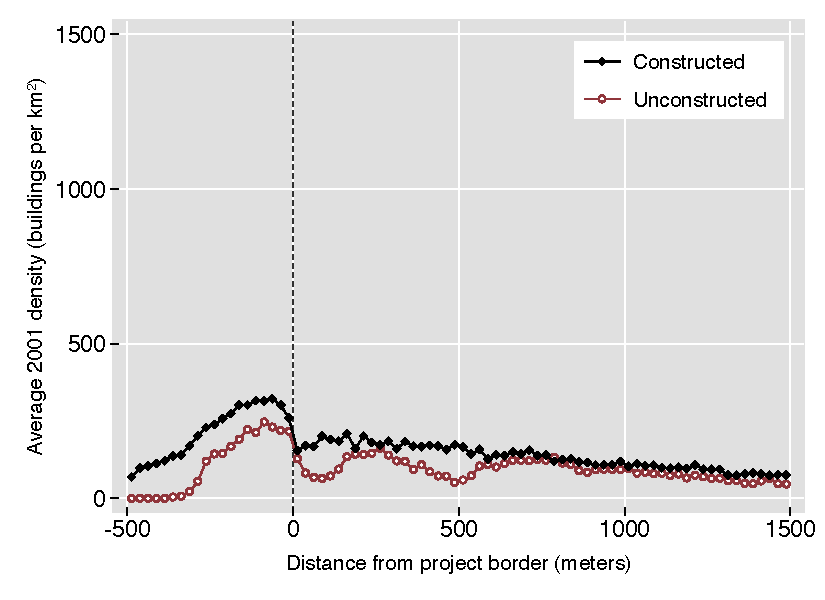
\includegraphics[width=\textwidth,trim={0.3cm .3cm 0.1cm 0cm}, clip=true]{figures/bblu_inf_pre_means_4_1_spk.pdf}

        \end{subfigure}
        \begin{subfigure}[b]{0.48\textwidth}
                    \caption[Network2]%
            {{\footnotesize \textbf{In-Situ} pre-period formal  raw data}}   
            \label{fig:prefor}
            \centering
            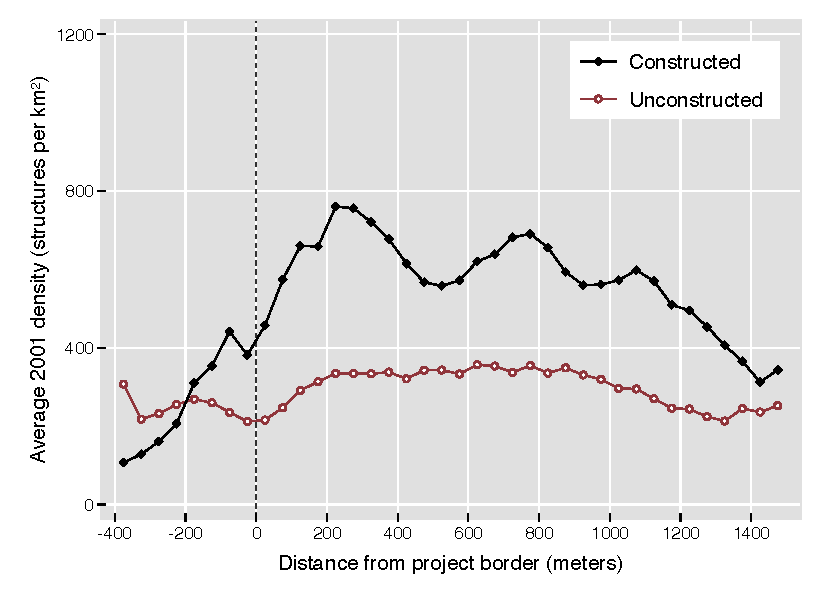
\includegraphics[width=\textwidth,trim={0.3cm .3cm 0.1cm 0cm}, clip=true]{figures/bblu_for_pre_means_4_2_spk.pdf}

        \end{subfigure}
        \hfill
        \begin{subfigure}[b]{0.48\textwidth}  
                    \caption[]%
            {{\footnotesize \textbf{In-Situ} pre-period informal  raw data}}     
            \label{fig:preinf}
            \centering 
            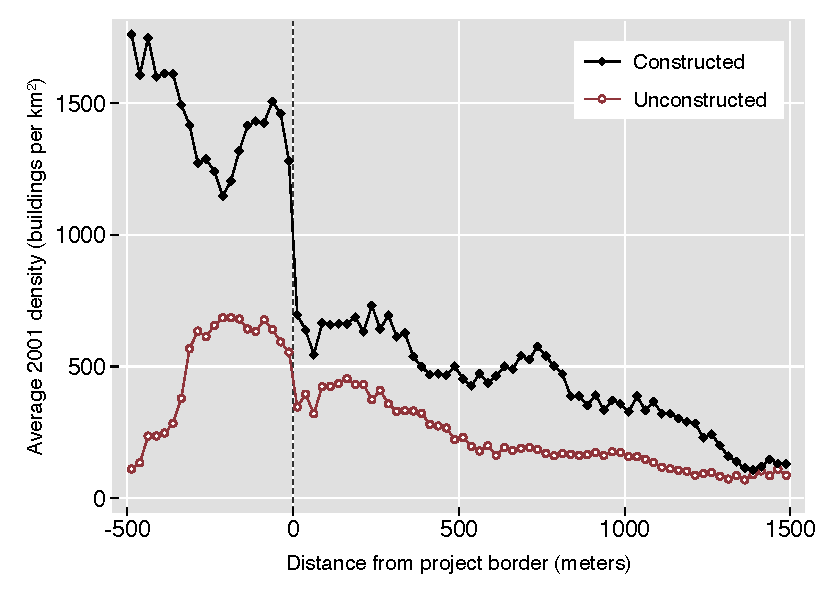
\includegraphics[width=\textwidth,trim={0.3cm .3cm 0.1cm 0cm}, clip=true]{figures/bblu_inf_pre_means_4_2_spk.pdf}

        \end{subfigure}
        \begin{subfigure}[b]{0.48\textwidth}
                    \caption[Network2]%
            {{\footnotesize \textbf{Other} pre-period formal  raw data}}   
            \label{fig:prefor}
            \centering
            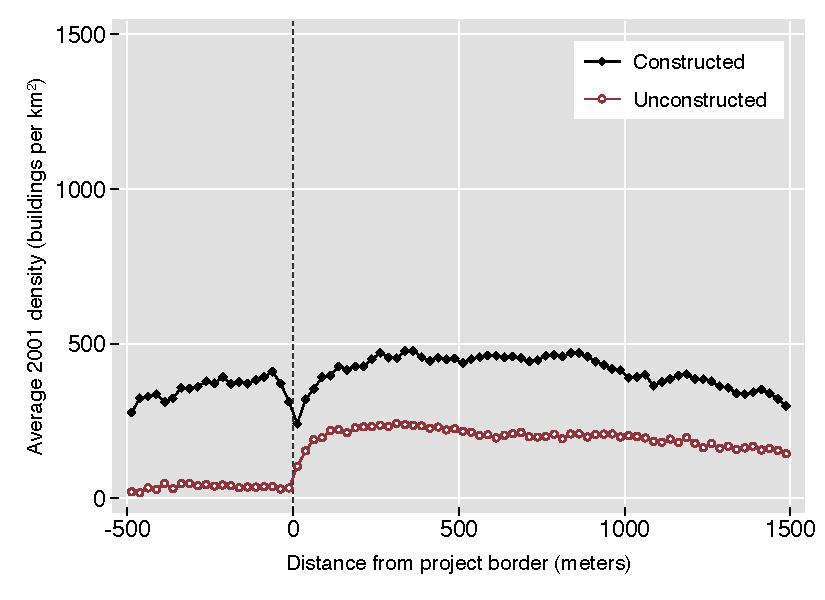
\includegraphics[width=\textwidth,trim={0.3cm .3cm 0.1cm 0cm}, clip=true]{figures/bblu_for_pre_means_4_3_spk.pdf}

        \end{subfigure}
        \hfill
        \begin{subfigure}[b]{0.48\textwidth}  
                    \caption[]%
            {{\footnotesize \textbf{Other} pre-period informal  raw data}}      
            \label{fig:preinf}
            \centering 
            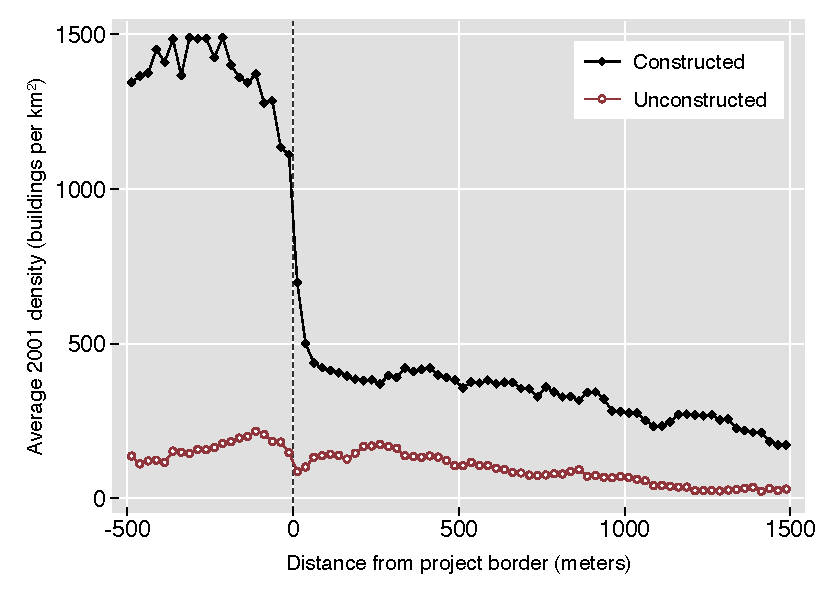
\includegraphics[width=\textwidth,trim={0.3cm .3cm 0.1cm 0cm}, clip=true]{figures/bblu_inf_pre_means_4_3_spk.pdf}

        \end{subfigure}
\end{figure*}


\begin{figure*}
        \centering
   %     \caption[ Pre-Period Housing Densities in Constructed and Unconstructed Projects Areas ]
  %      {\small Pre-Period Densities} 
        %\vspace{2mm}
        \begin{subfigure}[b]{0.48\textwidth}
                    \caption[Network2]%
            {{\footnotesize \textbf{All Projects} pre-period formal fe}}    
            \label{fig:prefor}
            \centering
            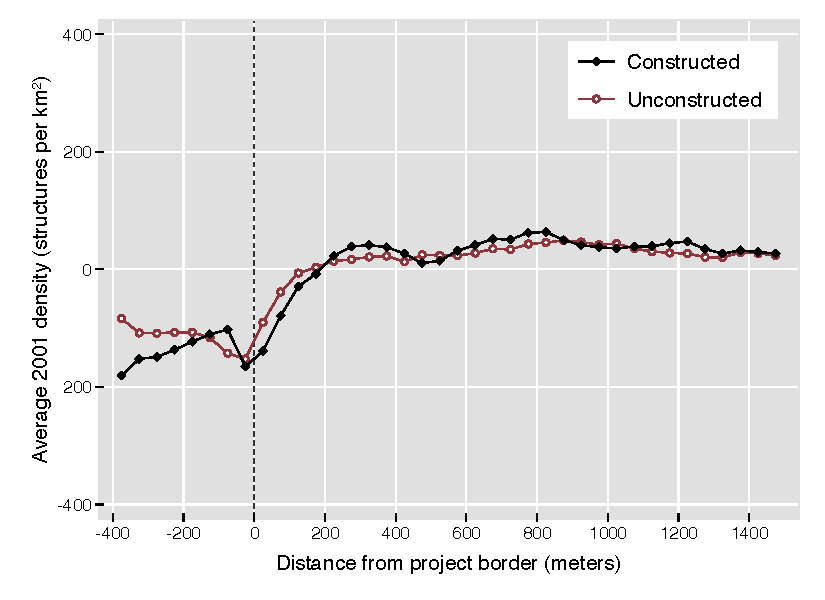
\includegraphics[width=\textwidth,trim={0.3cm .3cm 0.1cm 0cm}, clip=true]{figures/bblu_for_fe_pre_means_4_mpk.pdf}

        \end{subfigure}
        \hfill
        \begin{subfigure}[b]{0.48\textwidth}  
                    \caption[]%
            {{\footnotesize \textbf{All Projects} pre-period informal fe }}      
            \label{fig:preinf}
            \centering 
            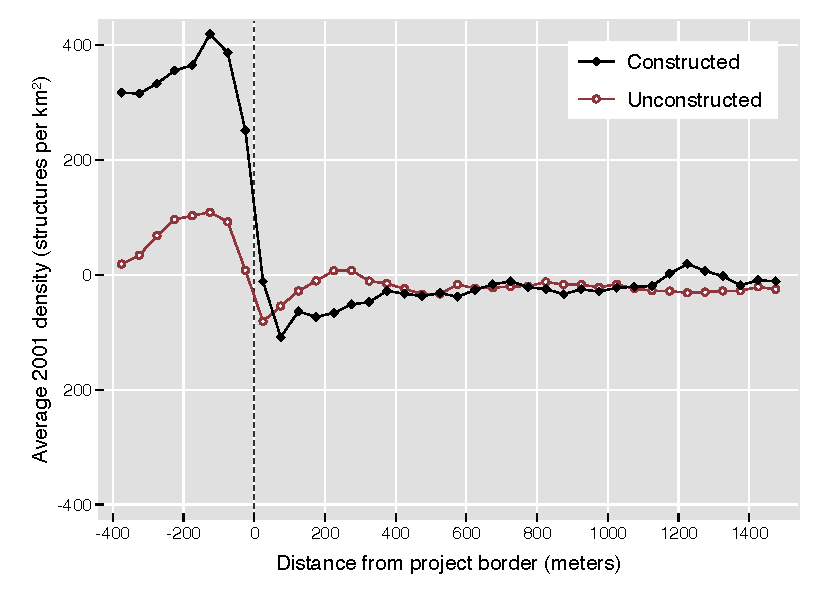
\includegraphics[width=\textwidth,trim={0.3cm .3cm 0.1cm 0cm}, clip=true]{figures/bblu_inf_fe_pre_means_4_mpk.pdf}

        \end{subfigure}
        \begin{subfigure}[b]{0.48\textwidth}
                    \caption[Network2]%
            {{\footnotesize \textbf{Greenfield} pre-period formal  fe }}    
            \label{fig:prefor}
            \centering
            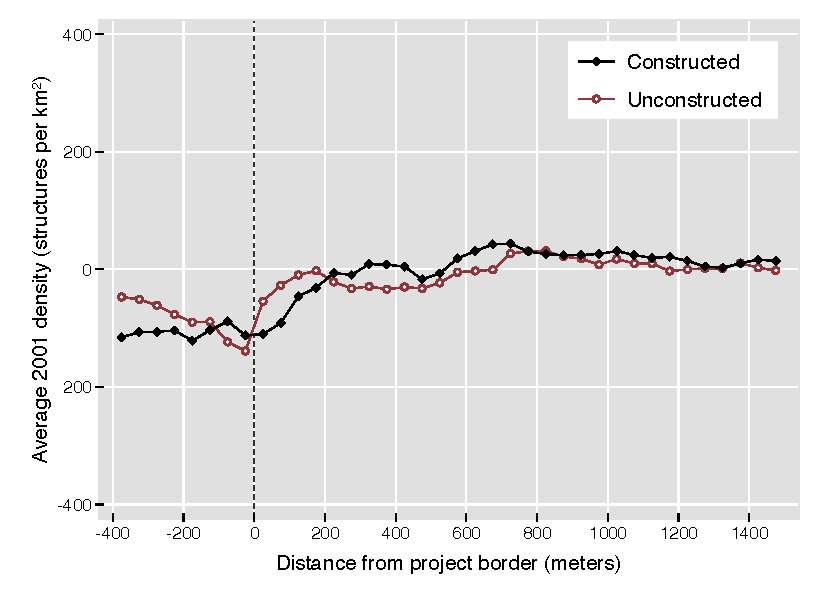
\includegraphics[width=\textwidth,trim={0.3cm .3cm 0.1cm 0cm}, clip=true]{figures/bblu_for_fe_pre_means_4_1_mpk.pdf}

        \end{subfigure}
        \hfill
        \begin{subfigure}[b]{0.48\textwidth}  
                    \caption[]%
            {{\footnotesize \textbf{Greenfield} pre-period informal fe }}     
            \label{fig:preinf}
            \centering 
            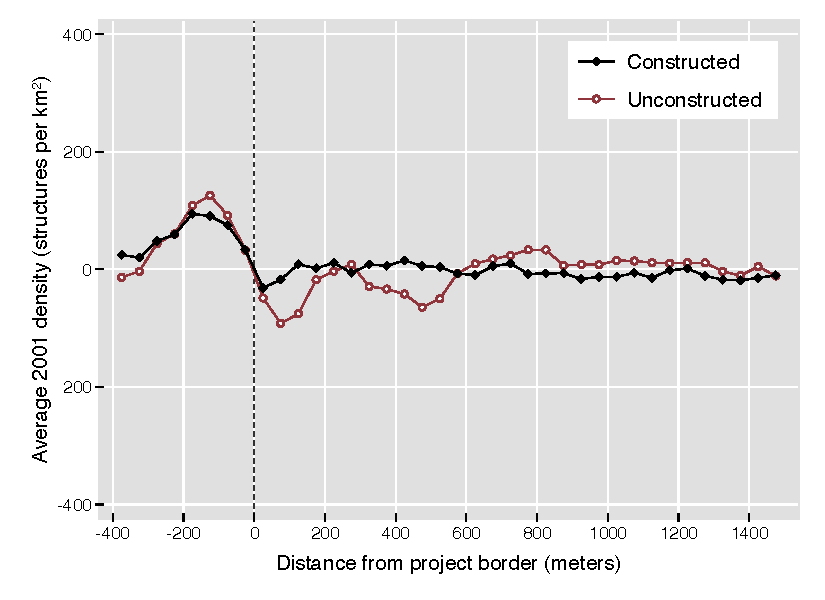
\includegraphics[width=\textwidth,trim={0.3cm .3cm 0.1cm 0cm}, clip=true]{figures/bblu_inf_fe_pre_means_4_1_mpk.pdf}

        \end{subfigure}
        \begin{subfigure}[b]{0.48\textwidth}
                    \caption[Network2]%
            {{\footnotesize \textbf{In-Situ} pre-period formal fe }}   
            \label{fig:prefor}
            \centering
            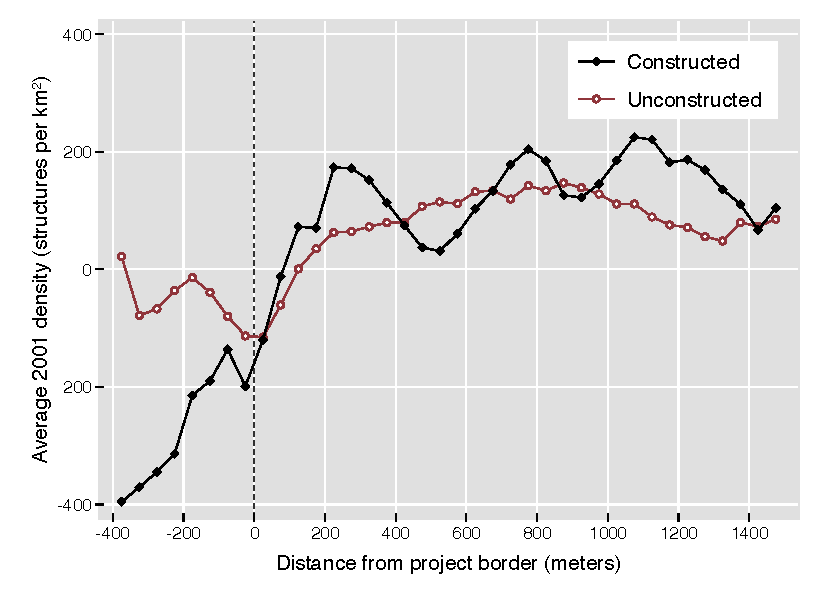
\includegraphics[width=\textwidth,trim={0.3cm .3cm 0.1cm 0cm}, clip=true]{figures/bblu_for_fe_pre_means_4_2_mpk.pdf}

        \end{subfigure}
        \hfill
        \begin{subfigure}[b]{0.48\textwidth}  
                    \caption[]%
            {{\footnotesize \textbf{In-Situ} pre-period informal fe }}     
            \label{fig:preinf}
            \centering 
            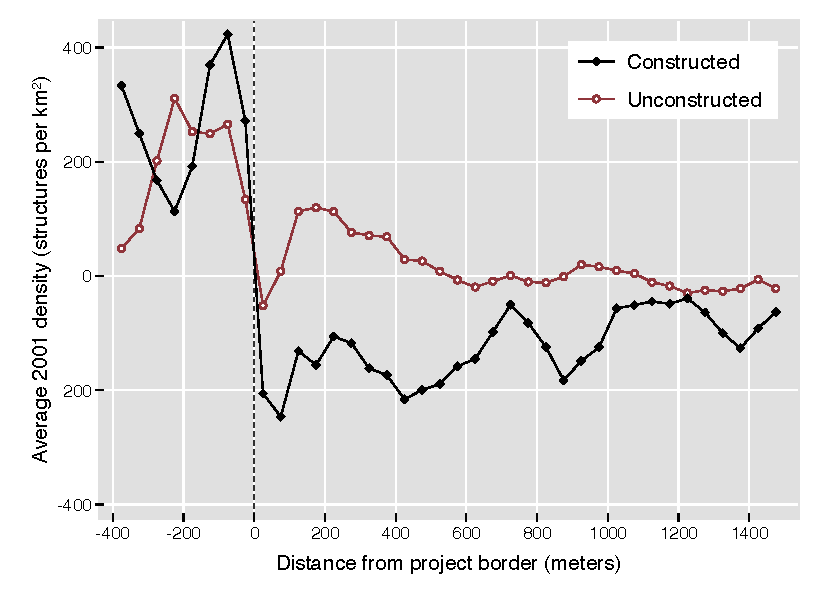
\includegraphics[width=\textwidth,trim={0.3cm .3cm 0.1cm 0cm}, clip=true]{figures/bblu_inf_fe_pre_means_4_2_mpk.pdf}

        \end{subfigure}
        \begin{subfigure}[b]{0.48\textwidth}
                    \caption[Network2]%
            {{\footnotesize \textbf{Other} pre-period formal fe }}   
            \label{fig:prefor}
            \centering
            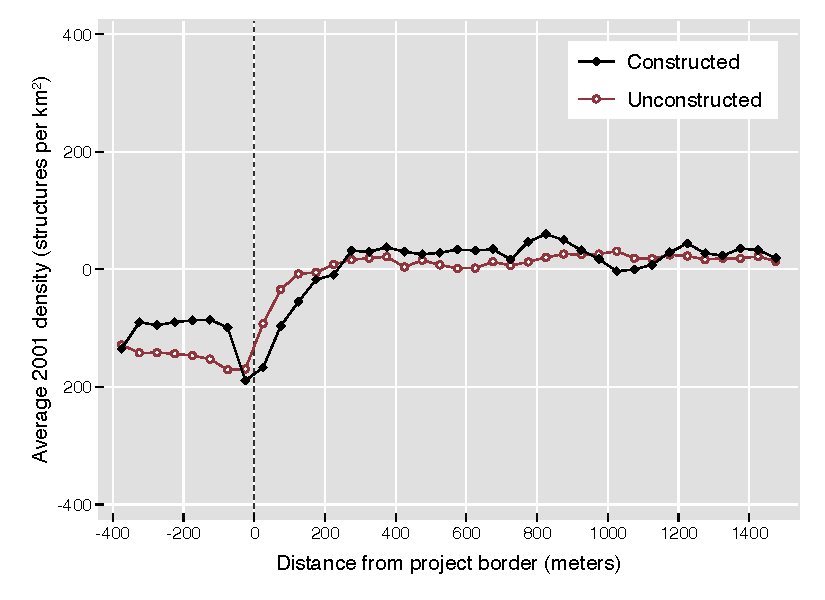
\includegraphics[width=\textwidth,trim={0.3cm .3cm 0.1cm 0cm}, clip=true]{figures/bblu_for_fe_pre_means_4_3_mpk.pdf}

        \end{subfigure}
        \hfill
        \begin{subfigure}[b]{0.48\textwidth}  
                    \caption[]%
            {{\footnotesize \textbf{Other} pre-period informal fe }}      
            \label{fig:preinf}
            \centering 
            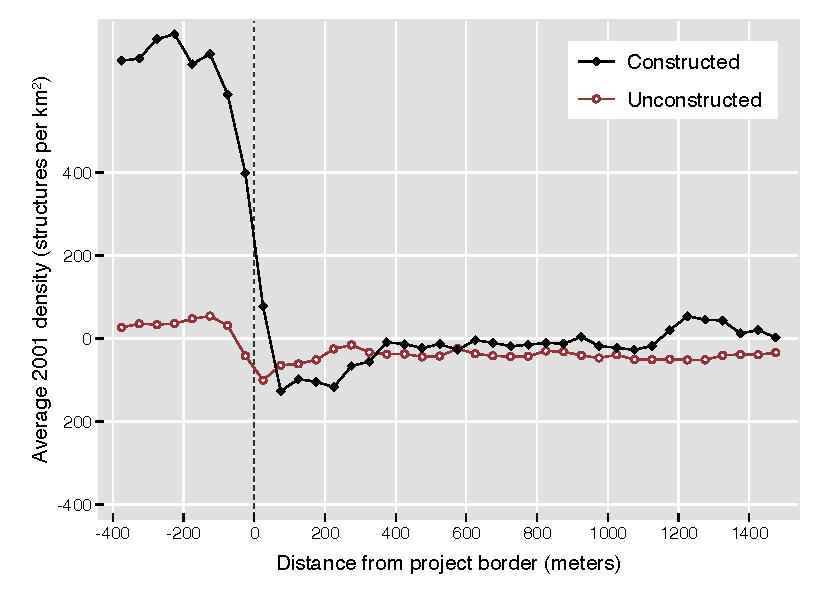
\includegraphics[width=\textwidth,trim={0.3cm .3cm 0.1cm 0cm}, clip=true]{figures/bblu_inf_fe_pre_means_4_3_mpk.pdf}

        \end{subfigure}
\end{figure*}








\begin{figure*}
        \centering
   %     \caption[ Pre-Period Housing Densities in Constructed and Unconstructed Projects Areas ]
  %      {\small Pre-Period Densities} 
        %\vspace{2mm}
        \begin{subfigure}[b]{0.48\textwidth}
            \caption[Network2]%
            {{\footnotesize \textbf{All Projects} changes formal raw data}}    
            \label{fig:prefor}
            \centering
            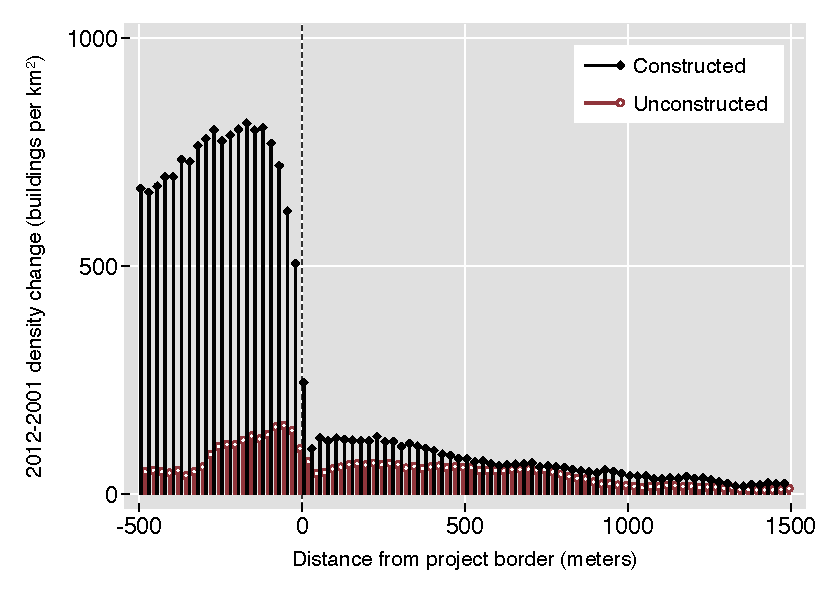
\includegraphics[width=\textwidth,trim={0.3cm .3cm 0.1cm 0cm}, clip=true]{figures/bblu_for_rawchanges_4_spk.pdf}

        \end{subfigure}
        \hfill
        \begin{subfigure}[b]{0.48\textwidth}  
                    \caption[]%
            {{\footnotesize \textbf{All Projects} changes informal  raw data}}      
            \label{fig:preinf}
            \centering 
            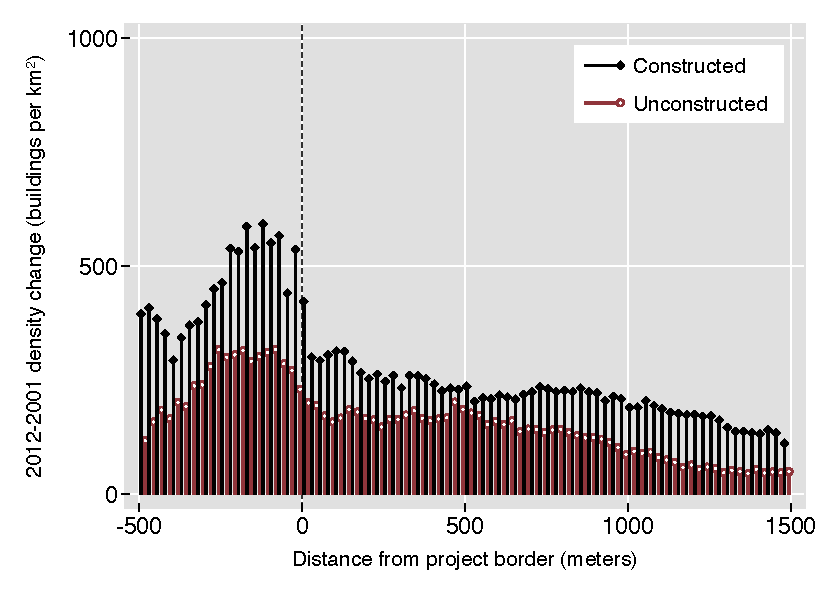
\includegraphics[width=\textwidth,trim={0.3cm .3cm 0.1cm 0cm}, clip=true]{figures/bblu_inf_rawchanges_4_spk.pdf}

        \end{subfigure}
        \begin{subfigure}[b]{0.48\textwidth}
                    \caption[Network2]%
            {{\footnotesize \textbf{Greenfield} changes formal  raw data}}    
            \label{fig:prefor}
            \centering
            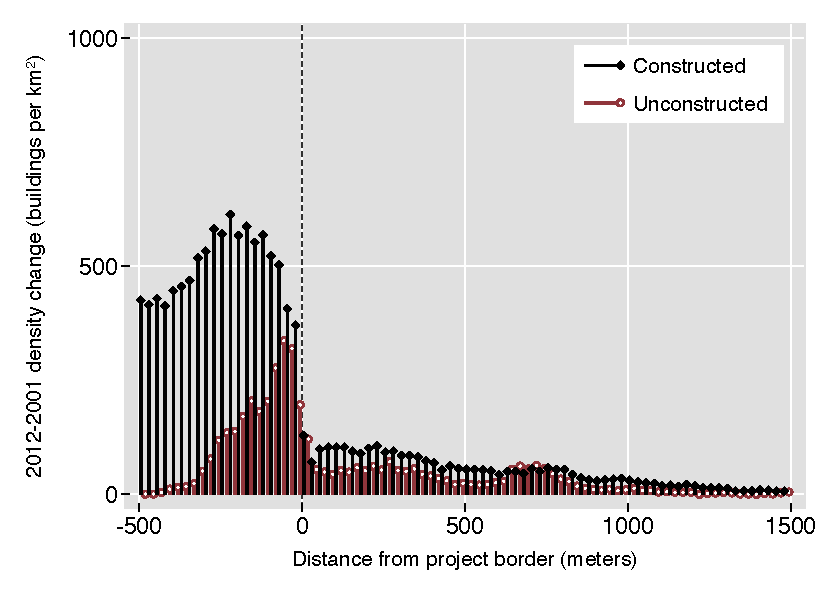
\includegraphics[width=\textwidth,trim={0.3cm .3cm 0.1cm 0cm}, clip=true]{figures/bblu_for_rawchanges_4_1_spk.pdf}

        \end{subfigure}
        \hfill
        \begin{subfigure}[b]{0.48\textwidth}  
                    \caption[]%
            {{\footnotesize \textbf{Greenfield} changes informal raw data }}     
            \label{fig:preinf}
            \centering 
            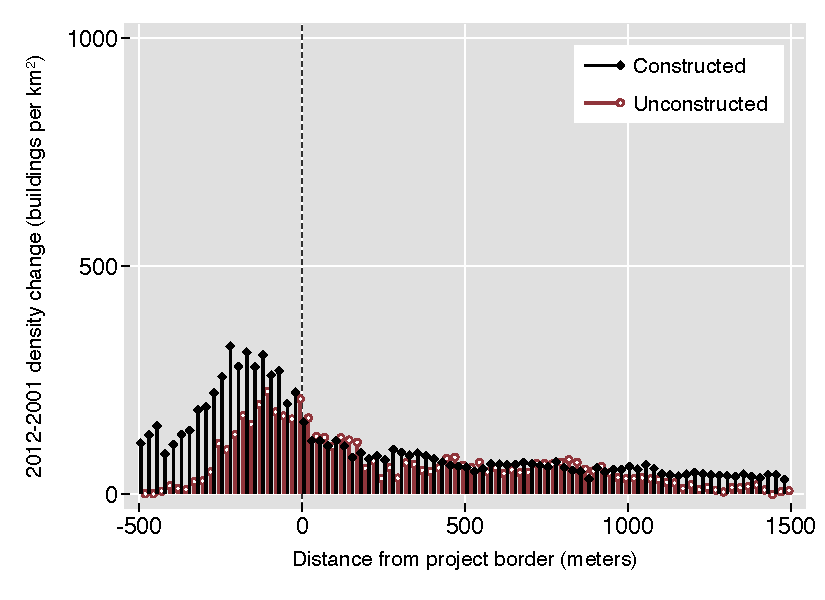
\includegraphics[width=\textwidth,trim={0.3cm .3cm 0.1cm 0cm}, clip=true]{figures/bblu_inf_rawchanges_4_1_spk.pdf}

        \end{subfigure}
        \begin{subfigure}[b]{0.48\textwidth}
                    \caption[Network2]%
            {{\footnotesize \textbf{In-Situ} changes formal raw data }}   
            \label{fig:prefor}
            \centering
            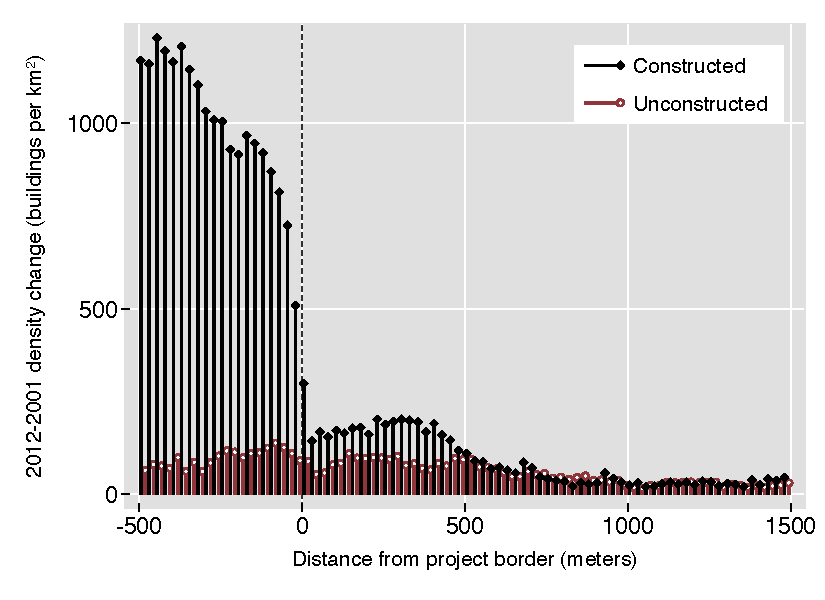
\includegraphics[width=\textwidth,trim={0.3cm .3cm 0.1cm 0cm}, clip=true]{figures/bblu_for_rawchanges_4_2_spk.pdf}

        \end{subfigure}
        \hfill
        \begin{subfigure}[b]{0.48\textwidth}  
                    \caption[]%
            {{\footnotesize \textbf{In-Situ} changes informal raw data }}     
            \label{fig:preinf}
            \centering 
            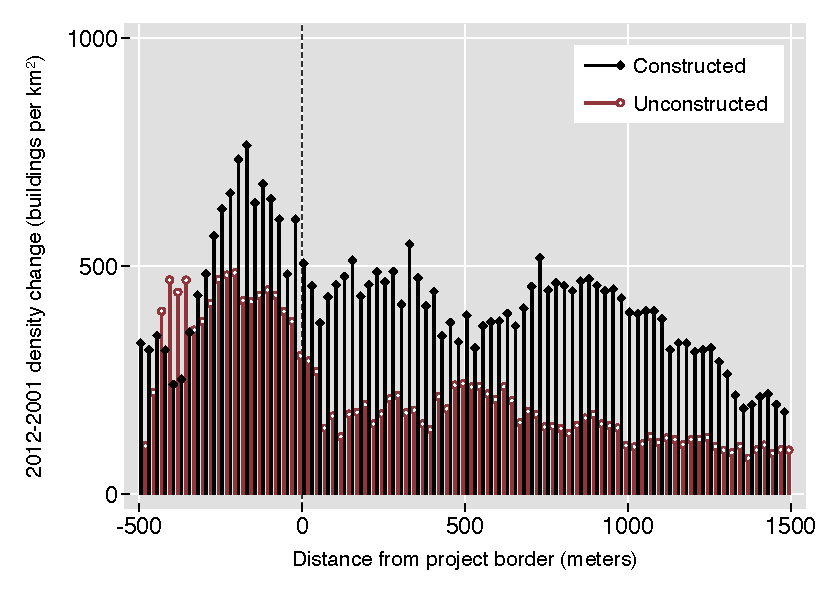
\includegraphics[width=\textwidth,trim={0.3cm .3cm 0.1cm 0cm}, clip=true]{figures/bblu_inf_rawchanges_4_2_spk.pdf}

        \end{subfigure}
        \begin{subfigure}[b]{0.48\textwidth}
                    \caption[Network2]%
            {{\footnotesize \textbf{Other} changes formal raw data}}   
            \label{fig:prefor}
            \centering
            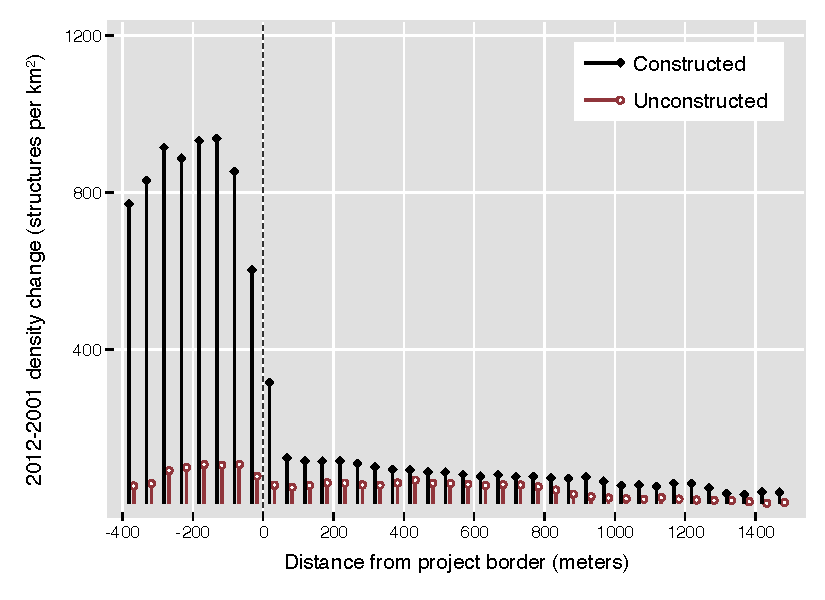
\includegraphics[width=\textwidth,trim={0.3cm .3cm 0.1cm 0cm}, clip=true]{figures/bblu_for_rawchanges_4_3_spk.pdf}

        \end{subfigure}
        \hfill
        \begin{subfigure}[b]{0.48\textwidth} 
                    \caption[]%
            {{\footnotesize \textbf{Other} changes informal  raw data}}      
            \label{fig:preinf} 
            \centering 
            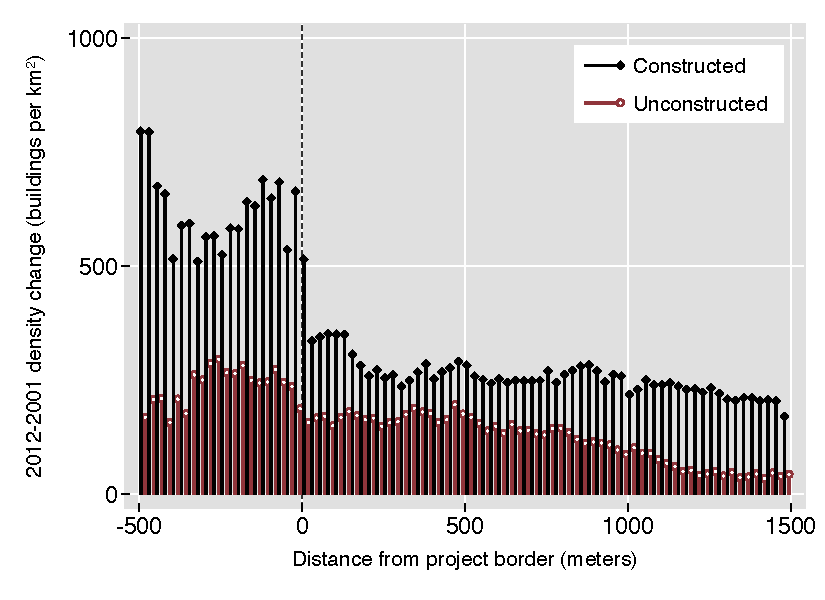
\includegraphics[width=\textwidth,trim={0.3cm .3cm 0.1cm 0cm}, clip=true]{figures/bblu_inf_rawchanges_4_3_spk.pdf}

        \end{subfigure}
\end{figure*}




\begin{figure*}
        \centering
   %     \caption[ Pre-Period Housing Densities in Constructed and Unconstructed Projects Areas ]
  %      {\small Pre-Period Densities} 
        %\vspace{2mm}
        \begin{subfigure}[b]{0.48\textwidth}
            \caption[Network2]%
            {{\footnotesize \textbf{All Projects} changes formal fe }}    
            \label{fig:prefor}
            \centering
            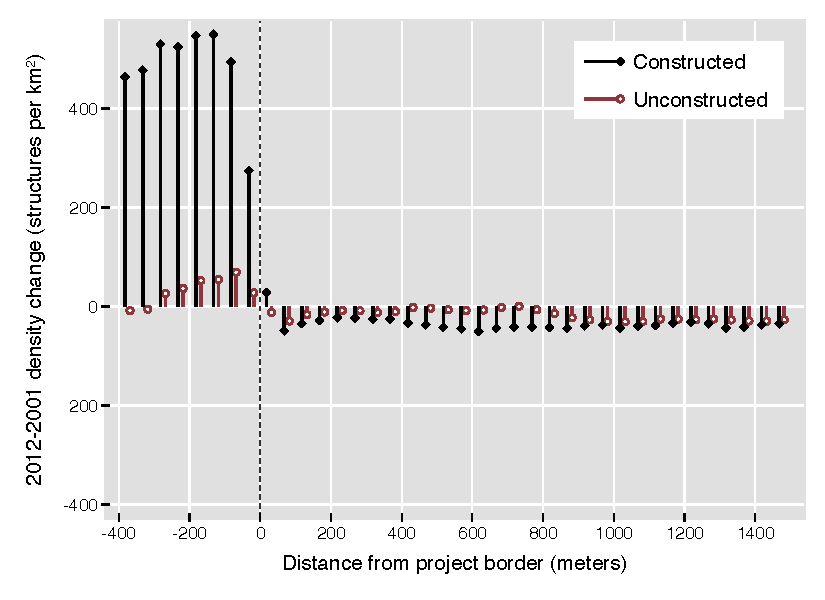
\includegraphics[width=\textwidth,trim={0.3cm .3cm 0.1cm 0cm}, clip=true]{figures/bblu_for_fe_rawchanges_4_mpk.pdf}

        \end{subfigure}
        \hfill
        \begin{subfigure}[b]{0.48\textwidth}  
                    \caption[]%
            {{\footnotesize \textbf{All Projects} changes informal  fe }}      
            \label{fig:preinf}
            \centering 
            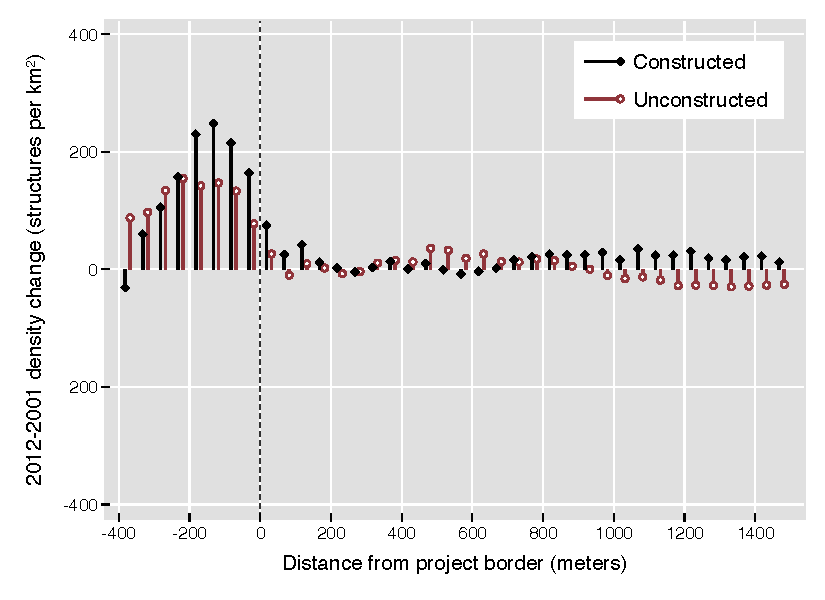
\includegraphics[width=\textwidth,trim={0.3cm .3cm 0.1cm 0cm}, clip=true]{figures/bblu_inf_fe_rawchanges_4_mpk.pdf}

        \end{subfigure}
        \begin{subfigure}[b]{0.48\textwidth}
                    \caption[Network2]%
            {{\footnotesize \textbf{Greenfield} changes formal  fe}}    
            \label{fig:prefor}
            \centering
            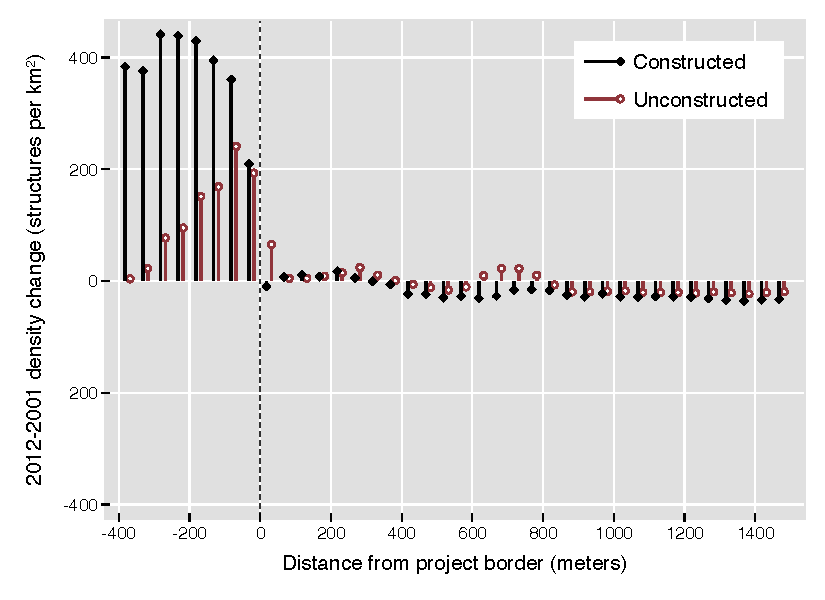
\includegraphics[width=\textwidth,trim={0.3cm .3cm 0.1cm 0cm}, clip=true]{figures/bblu_for_fe_rawchanges_4_1_mpk.pdf}

        \end{subfigure}
        \hfill
        \begin{subfigure}[b]{0.48\textwidth}  
                    \caption[]%
            {{\footnotesize \textbf{Greenfield} changes informal fe}}     
            \label{fig:preinf}
            \centering 
            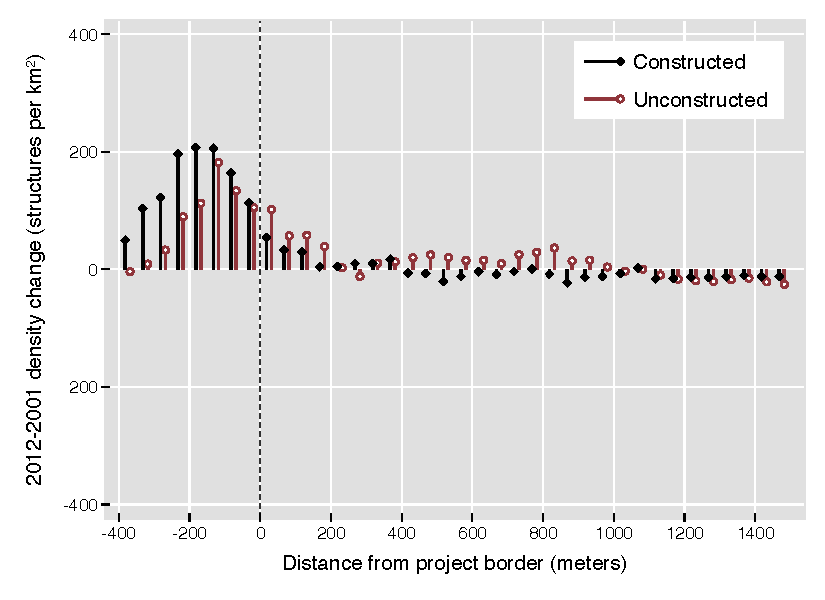
\includegraphics[width=\textwidth,trim={0.3cm .3cm 0.1cm 0cm}, clip=true]{figures/bblu_inf_fe_rawchanges_4_1_mpk.pdf}

        \end{subfigure}
        \begin{subfigure}[b]{0.48\textwidth}
                    \caption[Network2]%
            {{\footnotesize \textbf{In-Situ} changes formal fe}}   
            \label{fig:prefor}
            \centering
            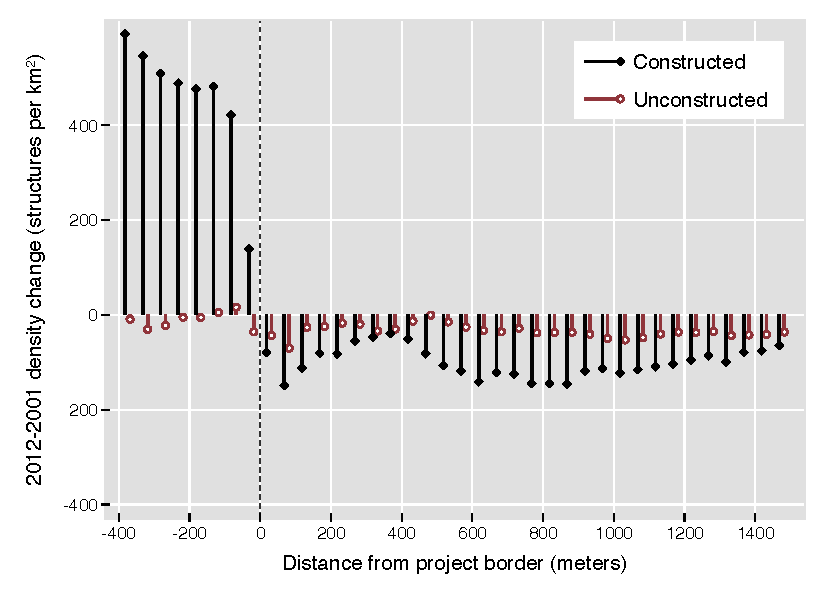
\includegraphics[width=\textwidth,trim={0.3cm .3cm 0.1cm 0cm}, clip=true]{figures/bblu_for_fe_rawchanges_4_2_mpk.pdf}

        \end{subfigure}
        \hfill
        \begin{subfigure}[b]{0.48\textwidth}  
                    \caption[]%
            {{\footnotesize \textbf{In-Situ} changes informal fe}}     
            \label{fig:preinf}
            \centering 
            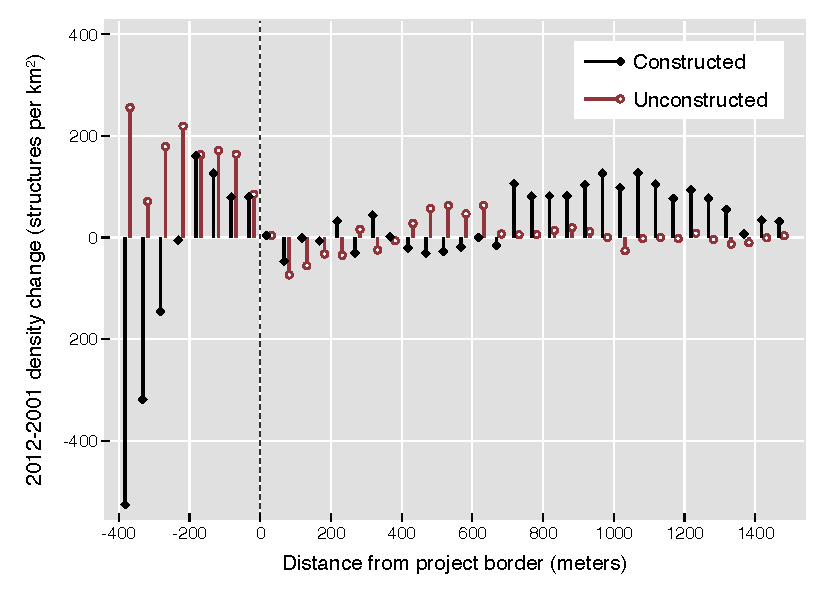
\includegraphics[width=\textwidth,trim={0.3cm .3cm 0.1cm 0cm}, clip=true]{figures/bblu_inf_fe_rawchanges_4_2_mpk.pdf}

        \end{subfigure}
        \begin{subfigure}[b]{0.48\textwidth}
                    \caption[Network2]%
            {{\footnotesize \textbf{Other} changes formal fe}}   
            \label{fig:prefor}
            \centering
            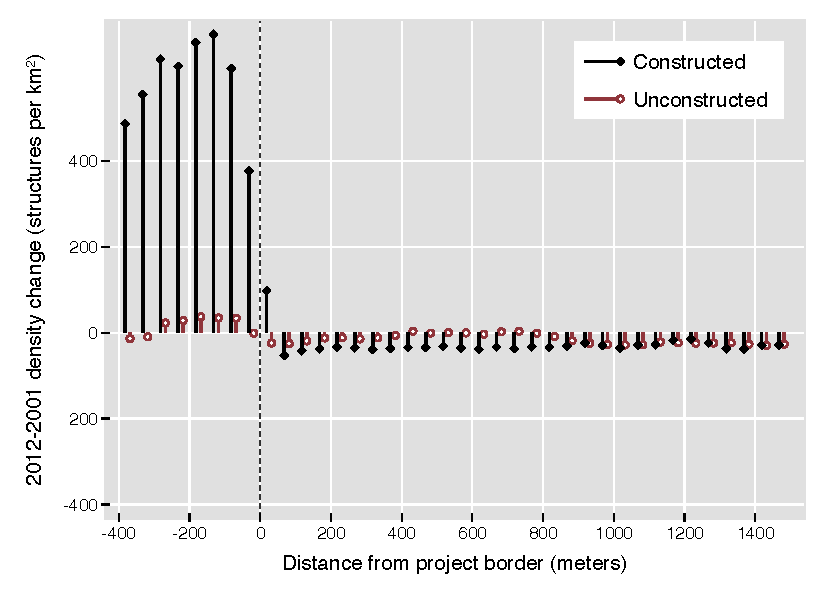
\includegraphics[width=\textwidth,trim={0.3cm .3cm 0.1cm 0cm}, clip=true]{figures/bblu_for_fe_rawchanges_4_3_mpk.pdf}

        \end{subfigure}
        \hfill
        \begin{subfigure}[b]{0.48\textwidth} 
                    \caption[]%
            {{\footnotesize \textbf{Other} changes informal  fe}}      
            \label{fig:preinf} 
            \centering 
            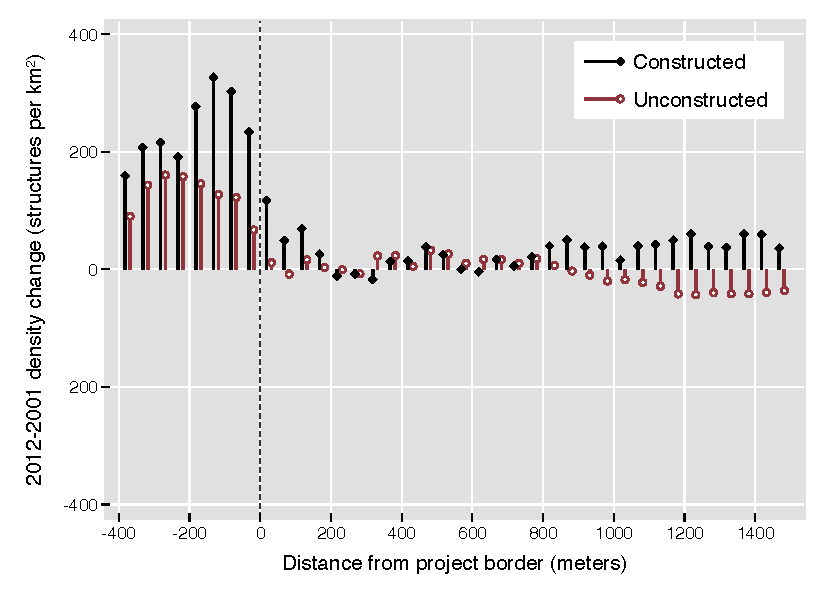
\includegraphics[width=\textwidth,trim={0.3cm .3cm 0.1cm 0cm}, clip=true]{figures/bblu_inf_fe_rawchanges_4_3_mpk.pdf}

        \end{subfigure}
\end{figure*}







\begin{table}
\caption{Building Density}
\begin{tabular}{lDDDDD}
\toprule
 & \small (1) & \small (2)  & \small (3) & \small (4) & \small (5) \\
 & Total & Formal  & Informal & Informal Bkyd. & Informal Non-Bkyd. \\ \midrule
\textbf{All Projects} \\inside project      &     649.922\textsuperscript{a}&     578.443\textsuperscript{a}&      71.480                   &     504.849\textsuperscript{a}&    -433.370\textsuperscript{a}\\
                    &   (142.586)                   &    (74.804)                   &   (109.401)                   &   (103.803)                   &    (87.274)                   \\[0.5em]
0-300m outside project &      -4.615                   &      34.561                   &     -39.176                   &       6.232                   &     -45.408                   \\
                    &    (43.548)                   &    (24.463)                   &    (35.468)                   &    (31.660)                   &    (28.680)                   \\[0.5em]
300-600m outside project &     -93.284\textsuperscript{b}&      -4.618                   &     -88.666\textsuperscript{a}&     -65.122\textsuperscript{b}&     -23.544                   \\
                    &    (37.620)                   &    (16.266)                   &    (33.160)                   &    (28.282)                   &    (16.891)                   \\[0.5em]
R$^2$               &       0.339                   &       0.284                   &       0.260                   &       0.230                   &       0.141                   \\

\midrule
\textbf{Greenfield} \\   inside project      &     353.183                   &     293.597\textsuperscript{b}&      59.586                   &     126.015                   &     -66.429                   \\
                    &   (230.338)                   &   (147.088)                   &   (112.815)                   &   (121.632)                   &    (58.470)                   \\[0.01em]
0-300m outside project &     -61.727                   &     -25.684                   &     -36.042                   &     -65.700                   &      29.657                   \\
                    &    (97.953)                   &    (47.498)                   &    (66.667)                   &    (60.153)                   &    (55.235)                   \\[0.01em]
300-600m outside project&     -58.151                   &     -22.320                   &     -35.831                   &     -34.795                   &      -1.036                   \\
                    &    (48.864)                   &    (24.476)                   &    (31.417)                   &    (21.621)                   &    (19.800)                   \\[0.8em] 
\textbf{In-Situ Upgrading} \\   inside project      &     591.912                   &     852.192\textsuperscript{a}&    -260.279                   &     657.640\textsuperscript{b}&    -917.919\textsuperscript{a}\\
                    &   (363.396)                   &   (147.464)                   &   (278.235)                   &   (270.994)                   &   (234.130)                   \\[0.01em]
0-300m outside project &      75.490                   &     130.970                   &     -55.481                   &      28.294                   &     -83.775                   \\
                    &   (152.824)                   &    (94.942)                   &   (111.397)                   &   (134.628)                   &    (98.608)                   \\[0.01em]
300-600m outside project &       8.443                   &     107.126                   &     -98.683                   &     -74.819                   &     -23.864                   \\
                    &   (101.978)                   &    (65.588)                   &    (83.895)                   &    (92.808)                   &    (72.003)                   \\[0.8em]
\textbf{Other} \\   inside project      &     869.317\textsuperscript{a}&     657.784\textsuperscript{a}&     211.533                   &     665.816\textsuperscript{a}&    -454.283\textsuperscript{a}\\
                    &   (178.797)                   &    (76.542)                   &   (146.943)                   &   (116.700)                   &   (102.134)                   \\[0.01em]
0-300m outside project &     -14.300                   &      31.301                   &     -45.601                   &       9.434                   &     -55.034                   \\
                    &    (68.395)                   &    (27.074)                   &    (57.967)                   &    (43.293)                   &    (38.193)                   \\[0.01em]
300-600m outside project &    -133.906\textsuperscript{a}&     -26.391                   &    -107.515\textsuperscript{b}&     -67.345\textsuperscript{c}&     -40.170\textsuperscript{c}\\
                    &    (50.456)                   &    (19.423)                   &    (45.582)                   &    (38.571)                   &    (20.745)                   \\[0.8em]
Mean Outcome 2001   &      379.90                   &      203.91                   &      175.98                   &       66.26                   &      109.72                   \\
Mean Outcome 2011   &      584.70                   &      281.66                   &      303.04                   &      192.77                   &      110.27                   \\
R$^2$               &       0.346                   &       0.287                   &       0.269                   &       0.237                   &       0.152                   \\
N                   &   2,721,910                   &   2,721,910                   &   2,721,910                   &   2,721,910                   &   2,721,910                   \\

\bottomrule
\end{tabular}
\end{table}





\begin{table}[h!] 
\caption{Effect of Housing Projects on Socio-demographics}
\label{table:sorting}
\small
\centering
%\caption{Census Composition Estimates }
\vspace{-2mm}
\begin{tabular}{lDDDDD}
\toprule
& \small (1) & \small (2) & \small (3) & \small (4)& \small (5)\\
& \small Age & \small P.O.B. not Gauteng & \small Unemployed & \small Years of Education & \small Monthly Income \\ \midrule 
\textbf{All Projects} \\inside project      &       0.038                   &      -0.021                   &       0.019                   &       0.259\textsuperscript{b}&    1678.766\textsuperscript{a}\\
                    &     (0.353)                   &     (0.024)                   &     (0.019)                   &     (0.125)                   &   (522.331)                   \\[0.5em]
0-300m outside project &       0.475                   &       0.018                   &       0.013                   &       0.172                   &     883.133                   \\
                    &     (0.329)                   &     (0.018)                   &     (0.018)                   &     (0.119)                   &   (538.551)                   \\[0.5em]
300-600m outside project &      -0.078                   &       0.009                   &       0.010                   &       0.045                   &     516.694                   \\
                    &     (0.336)                   &     (0.016)                   &     (0.016)                   &     (0.100)                   &   (510.868)                   \\[0.5em]
R$^2$               &       0.317                   &       0.469                   &       0.319                   &       0.492                   &       0.326                   \\

\midrule
\textbf{Greenfield} \\   inside project      &      -1.335\textsuperscript{c}&      -0.003                   &       0.090\textsuperscript{c}&      -0.205                   &     507.357                   \\
                    &     (0.753)                   &     (0.057)                   &     (0.047)                   &     (0.292)                   &   (830.382)                   \\[0.01em]
0-300m outside project &      -0.620                   &       0.062\textsuperscript{b}&       0.031                   &       0.018                   &     505.790                   \\
                    &     (0.700)                   &     (0.024)                   &     (0.050)                   &     (0.217)                   &   (675.641)                   \\[0.01em]
300-600m outside project&      -1.180\textsuperscript{c}&       0.078\textsuperscript{b}&       0.053                   &       0.315                   &    -151.795                   \\
                    &     (0.642)                   &     (0.034)                   &     (0.037)                   &     (0.252)                   &   (745.030)                   \\[0.8em] 
\textbf{In-Situ Upgrading} \\   inside project      &       0.331                   &      -0.047                   &      -0.005                   &       0.244                   &    1430.711                   \\
                    &     (0.731)                   &     (0.031)                   &     (0.028)                   &     (0.226)                   &  (1303.039)                   \\[0.01em]
0-300m outside project &       0.113                   &      -0.038                   &       0.025                   &       0.377                   &    1451.355                   \\
                    &     (0.751)                   &     (0.029)                   &     (0.031)                   &     (0.282)                   &  (1398.837)                   \\[0.01em]
300-600m outside project &      -0.985                   &       0.006                   &       0.033                   &      -0.194                   &    -857.690                   \\
                    &     (0.846)                   &     (0.029)                   &     (0.030)                   &     (0.257)                   &  (1210.921)                   \\[0.8em]
\textbf{Other} \\   inside project      &       0.246                   &       0.002                   &       0.018                   &       0.318                   &    2341.754\textsuperscript{a}\\
                    &     (0.598)                   &     (0.034)                   &     (0.028)                   &     (0.195)                   &   (744.384)                   \\[0.01em]
0-300m outside project &       1.078\textsuperscript{c}&       0.024                   &      -0.006                   &       0.133                   &    1095.453                   \\
                    &     (0.586)                   &     (0.029)                   &     (0.028)                   &     (0.155)                   &   (736.269)                   \\[0.01em]
300-600m outside project &       0.812                   &      -0.008                   &      -0.023                   &       0.102                   &    1611.720\textsuperscript{b}\\
                    &     (0.559)                   &     (0.029)                   &     (0.024)                   &     (0.159)                   &   (716.516)                   \\[0.8em]
Mean Outcome 2001   &       27.30                   &        0.37                   &        0.47                   &        8.26                   &    2,475.96                   \\
Mean Outcome 2011   &       28.30                   &        0.43                   &        0.33                   &        9.68                   &    4,486.48                   \\
R$^2$               &       0.323                   &       0.483                   &       0.324                   &       0.497                   &       0.333                   \\
N                   &      12,733                   &      12,726                   &      12,723                   &      12,727                   &      12,723                   \\

\bottomrule
\multicolumn{6}{l}{\footnotesize Standard errors clustered at the project level in parenthesis. \textsuperscript{c} p$<$0.10, \textsuperscript{b} p$<$0.05, \textsuperscript{a} p$<$0.01  }\\
\multicolumn{6}{l}{\footnotesize P.O.B. means ``place of birth.''  Monthly income is in Rands.}
\end{tabular}
\end{table}








\begin{landscape}
{\footnotesize

\begin{table}[]
\small
\centering
\caption{Census Household-level Estimates }\label{table:censusestimates}
\vspace{-2mm}
\resizebox{.9\linewidth}{!}{
\begin{tabular}{lDDDDDDDD}
\toprule
 & \small (1) & \small (2)  & \small (3) & \small (4) & \small (5)  & \small (6)  & \small (7) & (8)\\
 & \small Flush Toilet & \small Water Indoors  & \small Electricity Cooking & \small Electricity Heating & \small Electricity Lighting  & \small Number of Rooms  & \small Household Size & Population Density\\ \midrule 
\textbf{All Projects} \\inside project      &       0.117                   &       0.168\textsuperscript{a}&       0.215\textsuperscript{a}&       0.146\textsuperscript{b}&       0.094                   &       0.161                   &       0.112                   &   -1631.026                   \\
                    &     (0.077)                   &     (0.040)                   &     (0.077)                   &     (0.074)                   &     (0.081)                   &     (0.169)                   &     (0.106)                   &  (1506.509)                   \\[0.5em]
0-300m outside project &      -0.024                   &       0.027                   &       0.024                   &       0.018                   &      -0.007                   &       0.092                   &      -0.007                   &    -713.308                   \\
                    &     (0.041)                   &     (0.041)                   &     (0.039)                   &     (0.045)                   &     (0.035)                   &     (0.130)                   &     (0.060)                   &   (756.093)                   \\[0.5em]
300-600m outside project &       0.008                   &       0.038                   &       0.022                   &       0.028                   &       0.003                   &      -0.003                   &       0.011                   &   -1364.475                   \\
                    &     (0.029)                   &     (0.036)                   &     (0.030)                   &     (0.034)                   &     (0.028)                   &     (0.120)                   &     (0.060)                   &  (1015.548)                   \\[0.5em]
R$^2$               &       0.202                   &       0.272                   &       0.295                   &       0.302                   &       0.222                   &       0.285                   &       0.324                   &       0.387                   \\

\midrule
\textbf{Greenfield} \\   inside project      &       0.065                   &       0.157                   &       0.105                   &       0.039                   &       0.082                   &       0.352                   &       0.285                   &    2390.856                   \\
                    &     (0.145)                   &     (0.118)                   &     (0.122)                   &     (0.132)                   &     (0.129)                   &     (0.427)                   &     (0.205)                   &  (3780.426)                   \\[0.01em]
0-300m outside project &      -0.097                   &       0.035                   &      -0.078                   &      -0.054                   &      -0.043                   &       0.338                   &       0.245\textsuperscript{c}&    1512.192                   \\
                    &     (0.071)                   &     (0.097)                   &     (0.077)                   &     (0.084)                   &     (0.052)                   &     (0.291)                   &     (0.139)                   &  (1745.342)                   \\[0.01em]
300-600m outside project&       0.004                   &      -0.033                   &       0.005                   &      -0.011                   &       0.051                   &      -0.127                   &       0.026                   &    -430.600                   \\
                    &     (0.064)                   &     (0.073)                   &     (0.055)                   &     (0.061)                   &     (0.046)                   &     (0.225)                   &     (0.113)                   &  (2435.044)                   \\[0.8em] 
\textbf{In-Situ Upgrading} \\   inside project      &       0.336\textsuperscript{b}&       0.167\textsuperscript{c}&       0.221\textsuperscript{b}&       0.205\textsuperscript{b}&       0.116                   &       0.454                   &       0.298\textsuperscript{c}&   -4514.304                   \\
                    &     (0.154)                   &     (0.095)                   &     (0.104)                   &     (0.097)                   &     (0.099)                   &     (0.293)                   &     (0.178)                   &  (3430.383)                   \\[0.01em]
0-300m outside project &       0.010                   &       0.014                   &       0.042                   &       0.032                   &       0.018                   &       0.021                   &       0.122                   &   -1760.017                   \\
                    &     (0.098)                   &     (0.102)                   &     (0.083)                   &     (0.102)                   &     (0.071)                   &     (0.314)                   &     (0.105)                   &  (1681.614)                   \\[0.01em]
300-600m outside project &      -0.017                   &      -0.017                   &       0.015                   &       0.054                   &      -0.041                   &      -0.301                   &       0.041                   &     221.621                   \\
                    &     (0.067)                   &     (0.085)                   &     (0.074)                   &     (0.085)                   &     (0.064)                   &     (0.350)                   &     (0.100)                   &  (1574.700)                   \\[0.8em]
\textbf{Other} \\   inside project      &      -0.039                   &       0.191\textsuperscript{a}&       0.186\textsuperscript{c}&       0.109                   &       0.039                   &      -0.095                   &      -0.101                   &   -1749.712                   \\
                    &     (0.096)                   &     (0.061)                   &     (0.111)                   &     (0.104)                   &     (0.121)                   &     (0.263)                   &     (0.139)                   &  (1320.522)                   \\[0.01em]
0-300m outside project &      -0.022                   &       0.064                   &       0.027                   &       0.021                   &      -0.016                   &       0.162                   &      -0.134                   &   -1603.812                   \\
                    &     (0.048)                   &     (0.054)                   &     (0.047)                   &     (0.050)                   &     (0.044)                   &     (0.185)                   &     (0.087)                   &  (1109.921)                   \\[0.01em]
300-600m outside project &       0.023                   &       0.103\textsuperscript{c}&       0.038                   &       0.039                   &       0.015                   &       0.189                   &      -0.055                   &   -2850.050\textsuperscript{b}\\
                    &     (0.041)                   &     (0.056)                   &     (0.040)                   &     (0.041)                   &     (0.039)                   &     (0.179)                   &     (0.094)                   &  (1314.476)                   \\[0.8em]
Mean Outcome 2001   &        0.79                   &        0.35                   &        0.66                   &        0.62                   &        0.77                   &        3.30                   &        3.51                   &    8,566.83                   \\
Mean Outcome 2011   &        0.83                   &        0.54                   &        0.81                   &        0.72                   &        0.82                   &        3.56                   &        3.18                   &    9,823.82                   \\
R$^2$               &       0.222                   &       0.288                   &       0.314                   &       0.318                   &       0.246                   &       0.293                   &       0.338                   &       0.393                   \\
N                   &      12,732                   &      12,732                   &      12,732                   &      12,732                   &      12,732                   &      12,709                   &      12,730                   &      12,734                   \\

\bottomrule
\multicolumn{9}{l}{\footnotesize All regressions include 3km grid Fixed-Effects. Standard errors clustered at the project level in parenthesis. \textsuperscript{c} p$<$0.10,\textsuperscript{b} p$<$0.05,\textsuperscript{a} p$<$0.01 }
\end{tabular}
}
\end{table}

}
\end{landscape}




\begin{table}
\small
\centering
\caption{Triple Difference Estimates on Log-Prices}\label{table:priceDDD_het}
\vspace{-2mm}
\begin{tabular}{lCC}
\toprule
 & \small (1) & \small (2)  \\ \midrule 
 \textbf{All Projects} \\
 inside project      &      -0.325                   &      -0.318                   \\
                    &     (0.369)                   &     (0.369)                   \\[0.55em]
0-300m outside project &      -0.205                   &      -0.203                   \\
                    &     (0.151)                   &     (0.151)                   \\[0.5em]
300-600m outside project &      -0.217\textsuperscript{b}&      -0.216\textsuperscript{b}\\
                    &     (0.096)                   &     (0.097)                   \\[0.5em]
Lot Size Controls   &                               &  \checkmark                   \\
r2                  &        0.32                   &        0.32                   \\
N                   &      67,751                   &      67,751                   \\

 \midrule
\textbf{Greenfield} \\   inside project      &       0.270                   &       0.259                   \\
                    &     (0.220)                   &     (0.218)                   \\[0.01em]
0-300m outside project &       0.004                   &       0.010                   \\
                    &     (0.175)                   &     (0.175)                   \\[0.01em]
300-600m outside project&       0.034                   &       0.038                   \\
                    &     (0.159)                   &     (0.160)                   \\[0.8em]
\textbf{In-Situ Upgrading} \\   inside project      &      -0.119                   &      -0.099                   \\
                    &     (0.394)                   &     (0.396)                   \\[0.01em]
0-300m outside project &      -0.573\textsuperscript{c}&      -0.573\textsuperscript{c}\\
                    &     (0.318)                   &     (0.318)                   \\[0.01em]
300-600m outside project &      -0.436\textsuperscript{c}&      -0.437\textsuperscript{c}\\
                    &     (0.224)                   &     (0.224)                   \\[0.8em]
\textbf{Other} \\   inside project      &      -0.953\textsuperscript{b}&      -0.947\textsuperscript{b}\\
                    &     (0.414)                   &     (0.412)                   \\[0.01em]
0-300m outside project &      -0.206                   &      -0.205                   \\
                    &     (0.155)                   &     (0.155)                   \\[0.01em]
300-600m outside project &      -0.197                   &      -0.197                   \\
                    &     (0.121)                   &     (0.121)                   \\[0.8em]
Lot Size Controls   &                               &  \checkmark                   \\
r2                  &        0.33                   &        0.33                   \\
N                   &      67,751                   &      67,751                   \\

\bottomrule
\multicolumn{3}{l}{\footnotesize Standard errors clustered at the project level in parenthesis.} \\
\multicolumn{3}{l}{ \textsuperscript{c} p$<$0.10,\textsuperscript{b} p$<$0.05,\textsuperscript{a} p$<$0.01 }
\end{tabular}
\end{table} 

% \begin{figure}
% 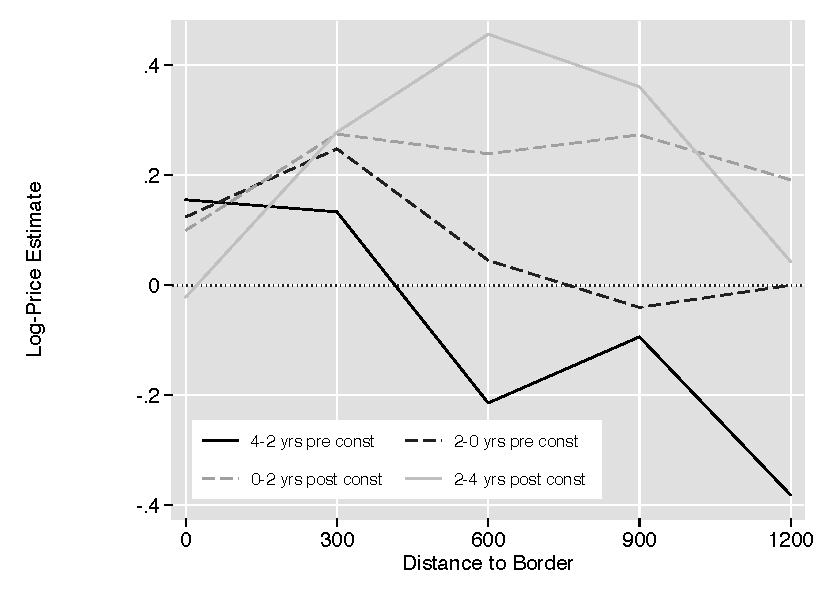
\includegraphics{figures/price_to_event_30.pdf}
% \end{figure}


\end{document}


